%%%%%%%%%%%%%%%%%%%%%%%%%%%%%%%%%%%%%%%%%%%%%%%%%%%%%%%%%%%%%%%%%%%%%%%%%%%%%%%%
\chapter{Building graphs without properties}
\label{sec:Building-graphs-without-properties}
%%%%%%%%%%%%%%%%%%%%%%%%%%%%%%%%%%%%%%%%%%%%%%%%%%%%%%%%%%%%%%%%%%%%%%%%%%%%%%%%

Boost.Graph is about creating graphs.
In this chapter we create the simplest of graphs, in which edges and nodes
have no properties (e.g. having a name).

Still, there are two types of graphs that can be constructed: undirected
and directed graphs.
The difference between directed and undirected graphs is in the edges:
in an undirected graph, 
an edge connects two vertices without any directionality, as displayed
in figure \ref{fig:undirected_graph_example}.

In a directed graph, an edge goes from a certain vertex, 
its source, to another (which may actually be the same), its target.
A directed graph is shown in figure \ref{fig:directed_graph_example}.

\begin{figure}
  \begin{tikzpicture}
    \draw[thick] 
      (0,0) node[draw=black,fill=white,shape=circle,text=white] {} 
      -- (5,2) node[draw=black,fill=white,shape=circle,text=white] {} 
      -- (10,1) node[draw=black,fill=white,shape=circle,text=white] {} 
    ;
  \end{tikzpicture}
  \caption{Example of an undirected graph}
  \label{fig:undirected_graph_example}
\end{figure}

\begin{figure}
  \begin{tikzpicture}
    \SetGraphUnit{5}
    \tikzset{VertexStyle/.append style = {draw=black,fill=white,shape=circle,text=white} }
    \Vertex{A}
    \EA(A){B}
    \EA(B){C}
    \tikzset{EdgeStyle/.append style = {->, bend left} }
    \Edge[](A)(B)
    \Edge[](B)(A)
    \Loop[dist = 4cm, dir = NO](A.west)
    \tikzset{EdgeStyle/.append style = {bend left = 0} }
    \Edge[](C)(B)   
  \end{tikzpicture}
  \caption{Example of a directed graph}
  \label{fig:directed_graph_example}
\end{figure}

In this chapter, we will build two directed and two undirected graphs:

\begin{itemize}
  \item An empty (directed) graph, which is the default type: 
    see chapter \ref{subsec:create_empty_directed_graph}
  \item An empty (undirected) graph: 
    see chapter \ref{subsec:create_empty_undirected_graph}
  \item A two-state Markov chain, a directed graph with two vertices 
    and four edges:
    see chapter \ref{subsec:create_markov_chain_graph}
  \item $K_{2}$, an undirected graph with two vertices and one edge, 
    see chapter \ref{subsec:create_k2_graph}
\end{itemize}


Creating an empty graph may sound trivial, it is not, thanks to the versatility
of the Boost.Graph library.

In the process of creating graphs, some basic (sometimes bordering trivial)
functions are encountered:

\begin{itemize}
  \item Counting the number of vertices, 
    see chapter \ref{subsec:get_n_vertices}
  \item Counting the number of edges,
     see chapter \ref{subsec:get_n_edges}
  \item Adding a vertex,
     see chapter \ref{subsec:add_vertex}
  \item Getting all vertices,
     see chapter \ref{subsec:get_vertices}
  \item Getting all vertex descriptors,
     see chapter \ref{subsec:get_vertex_descriptors}
  \item Adding an edge,
     see chapter \ref{subsec:add_edge}
  \item Getting all edges,
    see chapter \ref{subsec:get_edge_iterators}
  \item Getting all edge descriptors,
    see chapter \ref{subsec:get_edge_descriptors}
\end{itemize}

These functions are mostly there for completion and showing which data types
are used.

The chapter also introduces some important concepts:

\begin{itemize}
  \item Vertex descriptors,
    see chapter \ref{subsec:Vertex-descriptors}
  \item Edge insertion result,
    see chapter \ref{subsec:add_edge}
  \item Edge descriptors,
    see chapter \ref{subsec:Edge-descriptors}
\end{itemize}

After this chapter you may want to:

\begin{itemize}
  \item Building graphs with named vertices, 
    see chapter \ref{sec:Building-graphs-with-named-vertices}
  \item Building graphs with bundled vertices, 
    see chapter \ref{sec:Building-graphs-with-bundled-vertices}
  \item Building graphs with custom vertices,
    see chapter \ref{sec:Building-graphs-with-custom-properties}
  \item Building graphs with a graph name,
    see chapter \ref{sec:Building-graphs-with-a-graph-name}
\end{itemize}

%%%%%%%%%%%%%%%%%%%%%%%%%%%%%%%%%%%%%%%%%%%%%%%%%%%%%%%%%%%%%%%%%%%%%%%%%%%%%%%%
\section{Creating an empty (directed) graph}
\label{subsec:create_empty_directed_graph}
%%%%%%%%%%%%%%%%%%%%%%%%%%%%%%%%%%%%%%%%%%%%%%%%%%%%%%%%%%%%%%%%%%%%%%%%%%%%%%%%

Let's create an empty graph! 
Listing \ref{lst:create_empty_directed_graph} 
shows the function to create an empty graph.

\lstinputlisting[
  caption = Creating an empty (directed) graph,
  label = lst:create_empty_directed_graph
]{create_empty_directed_graph.impl}

The code consists out of an \verb;#include; and a function definition.
The \verb;#include; tells the compiler 
to read the header file \verb;adjacency_list.hpp;.
A header file (often with a \verb;.h; or \verb;.hpp; extension) 
contains class and functions declarations and/or definitions.
The header file \verb;adjacency_list.hpp; contains the 
\verb;boost::adjacency_list; class definition.
Without including this file, you will get compile errors like 
\verb;definition of boost::adjacency_list; unknown;
\footnote{
  In practice, these compiler error messages will be longer, bordering the unreadable
}. 

The function \verb;create_empty_directed_graph; has:

\begin{itemize}
  \item a return type: 
    The return type is \verb;boost::adjacency_list<>;, 
    that is a \verb;boost::adjacency_list; 
    with all template arguments set at their defaults
  \item a \verb;noexcept; specification: 
    the function should not throw
    \footnote{
      if the function would throw because it cannot allocate this little piece
      of memory, you are already in big trouble
    }, so it is preferred to mark it \verb;noexcept; 
    (\cite{stroustrup2013}, chapter 13.7)
  \item a function body: 
    all the function body does is implicitly create its return
    type by using the \verb;{};.
    An alternative syntax would be \verb;return boost::adjacency_list<>();,
    which is needlessly longer
\end{itemize}

Listing \ref{lst:create_empty_directed_graph_demo}
demonstrates the \verb;create_empty_directed_graph; function.
This demonstration is embedded within a Boost.Test unit test case.
It includes a Boost.Test header to allow to use the Boost.Test framework.
Additionally, a header file is included with the same name as the function
\footnote{
  I do not think it is important to have creative names
}.
This allows use to be able to use the function.
The test case creates an empty graph and stores it.
Instead of specifying the data type explicitly, 
\verb;auto; \index{auto} is used (this is preferred, \cite{stroustrup2013}
chapter 31.6), which lets the compiler figure out the type itself.

\lstinputlisting[
  caption = Demonstration of create\_empty\_directed\_graph,
  label = lst:create_empty_directed_graph_demo
]{create_empty_directed_graph_demo.impl}

Congratulations, you've just created a 
\verb;boost::adjacency_list; \index{boost::adjacency\_list}
with its default template arguments.
The \verb;boost::adjacency_list; is the most commonly used graph type, the other
is the \verb;boost::adjacency_matrix; \index{boost::adjacency\_matrix}.

We do not do anything with it yet, but still, you've just created a graph,
in which:

\begin{itemize}
  \item The out edges and vertices are stored in a \verb;std::vector; \index{std::vector}
  \item The edges have a direction
  \item The vertices, edges and graph have no properties
  \item The edges are stored in a \verb;std::list; \index{std::list}
\end{itemize}

It stores its edges, out edges and vertices in two different STL \index{STL}
\footnote{
  Standard Template Library, the standard library
}
containers.
std::vector \index{std::vector} is the container you should use by default (
  \cite{stroustrup2013}, chapter 31.6, 
  \cite{sutter_and_alexandrescu2004}, chapter 76
), as it has constant time look-up and back insertion.
The \verb;std::list; \index{std::list}
is used for storing the edges, as it is better suited at inserting elements
at any position.

I use \verb;const; \index{const} to store the empty graph as we do not modify it.
Correct use of \verb;const; is called const-correct.
Prefer to be const-correct \index{const-correctness}
(
  \cite{stroustrup1997}, chapter 7.9.3, 
  \cite{stroustrup2013}, chapter 12.7, 
  \cite{meyers2005effective}, item 3, 
  \cite{hollingworth2000cpp_builder_dev_guide}, chapter 3, 
  \cite{sutter_and_alexandrescu2004}, item 15, 
  \cite{cline1998cpp_faqs}, FAQ 14.05, 
  \cite{eckel2002thinking_cpp}, item 8, 
  \cite{lakos1996large}, 9.1.6
).

%%%%%%%%%%%%%%%%%%%%%%%%%%%%%%%%%%%%%%%%%%%%%%%%%%%%%%%%%%%%%%%%%%%%%%%%%%%%%%%%
\section{Creating an empty undirected graph}
\label{subsec:create_empty_undirected_graph}
\index{Create an empty graph}
\index{Empty graph, create}
\index{Create empty undirected graph}
%%%%%%%%%%%%%%%%%%%%%%%%%%%%%%%%%%%%%%%%%%%%%%%%%%%%%%%%%%%%%%%%%%%%%%%%%%%%%%%%

Let's create another empty graph! This time, we even make it undirected!
Listing \ref{lst:create_empty_undirected_graph}
shows how to create an undirected graph.

\lstinputlisting[
  caption = Creating an empty undirected graph,
  label = lst:create_empty_undirected_graph
]{create_empty_undirected_graph.impl}

This algorithm differs from the \verb;create_empty_directed_graph;
function (algorithm 
\ref{lst:create_empty_directed_graph}
) 
in that there are three template arguments that need to be specified in
the creation of the \verb;boost::adjacency_list;:

\begin{itemize}
  \item the first \verb;boost::vecS; \index{boost::vecS}: 
    select (that is what the \verb;S; \index{S}
    means) that out edges are stored in a std::vector.
    This is the default way.
  \item
    the second \verb;boost::vecS; \index{boost::vecS}: 
    select that the graph vertices are stored in a std::vector.
    This is the default way.
  \item
    \verb;boost::undirectedS; \index{boost::undirectedS}: 
    select that the graph is undirected.
    This is all we needed to change.
    By default, this argument is boost::directed \index{boost::directedS}
\end{itemize}

Listing \ref{lst:create_empty_undirected_graph_demo}
demonstrates the \verb;create_empty_undirected_graph; function.

\lstinputlisting[
  caption = Demonstration of create\_empty\_undirected\_graph,
  label = lst:create_empty_undirected_graph_demo
]{create_empty_undirected_graph_demo.impl}

Congratulations, with algorithm \ref{lst:create_empty_undirected_graph_demo}, 
you have just created an undirected graph in which:

\begin{itemize}
  \item The out edges and vertices are stored in a std::vector
  \item The graph is undirected
  \item Vertices, edges and graph have no properties
  \item Edges are stored in a std::list
\end{itemize}

%%%%%%%%%%%%%%%%%%%%%%%%%%%%%%%%%%%%%%%%%%%%%%%%%%%%%%%%%%%%%%%%%%%%%%%%%%%%%%%%
\section{Counting the number of vertices}
\label{subsec:get_n_vertices}
\index{Vertices, counting}
\index{Counting the number of vertices}
\index{Number of vertices, get}
\index{Get n vertices}
%%%%%%%%%%%%%%%%%%%%%%%%%%%%%%%%%%%%%%%%%%%%%%%%%%%%%%%%%%%%%%%%%%%%%%%%%%%%%%%%

Let's count all zero vertices of an empty graph!

\lstinputlisting[
  caption = Count the number of vertices,
  label = lst:get_n_vertices
]{get_n_vertices.impl}

The function \verb;get_n_vertices; takes the result of \verb;boost::num_vertices;
\index{boost::num\_vertices}, converts it to int and checks if there was conversion error.
We do so, as one should prefer using signed data types over unsigned ones
in an interface (\cite{lakos1996large}, chapter 9.2.2).
To do so, in the function body its first statement, 
the unsigned long \index{unsigned long}
produced by \verb;boost::num_vertices; \index{boost::num\_vertices}
get converted to an int using a \verb;static_cast; \index{static\_cast}.

Using an unsigned integer over a (signed) integer for the sake of gaining
that one more bit (\cite{stroustrup1997}, chapter 4.4) should be avoided.
The integer \verb;n; is initialized using list-initialization, which is preferred
over the other initialization syntaxes (\cite{stroustrup2013}, chapter 17.7.6).

The \verb;assert; checks if the conversion back to unsigned long re-creates the
original value, to check if no information has been lost.
If information is lost, the program crashes.
Use \verb;assert; \index{assert} extensively 
(\cite{stroustrup1997}, chapter 24.5.18, 
\cite{stroustrup2013}, chapter 30.5, 
\cite{sutter_and_alexandrescu2004}. chapter 68, 
\cite{mcconnell2004code}, chapter 8.2, 
\cite{liberty2001sams}, hour 24, 
\cite{lakos1996large}, chapter 2.6).

The function \verb;get_n_vertices; is demonstrated in algorithm 
\ref{lst:get_n_vertices_demo}, 
to measure the number of vertices of both the directed and undirected
graph we are already able to create.

\lstinputlisting[
  caption = Demonstration of the get\_n\_vertices function,
  label = lst:get_n_vertices_demo
]{get_n_vertices_demo.impl}

Note that the type of graph does not matter here.
One can count the number of vertices of every graph, as all graphs have
vertices.
Boost.Graph is very good at detecting operations that are not allowed, during
compile time.

%%%%%%%%%%%%%%%%%%%%%%%%%%%%%%%%%%%%%%%%%%%%%%%%%%%%%%%%%%%%%%%%%%%%%%%%%%%%%%%%
\section{Counting the number of edges}
\label{subsec:get_n_edges}
\index{Edges, counting}
\index{Counting the number of edges}
\index{Number of edges, get}
\index{Get n edges}
%%%%%%%%%%%%%%%%%%%%%%%%%%%%%%%%%%%%%%%%%%%%%%%%%%%%%%%%%%%%%%%%%%%%%%%%%%%%%%%%

Let's count all zero edges of an empty graph!

This is very similar to the previous chapter, 
only it uses \verb;boost::num_edges; \index{boost::num\_edges}
instead:

\lstinputlisting[
  caption = Count the number of edges,
  label = lst:get_n_edges
]{get_n_edges.impl}

This code is similar to the \verb;get_n_vertices; 
function (algorithm \ref{lst:get_n_vertices}, see rationale there) 
except \verb;boost::num_edges; \index{boost::num\_edges}
is used, instead of \verb;boost::num_vertices;, 
which also returns an unsigned long.

The function \verb;get_n_edges; is demonstrated in algorithm 
\ref{lst:get_n_edges_demo}, 
to measure the number of edges of an empty directed and undirected graph.

\lstinputlisting[
  caption = Demonstration of the get\_n\_edges function,
  label = lst:get_n_edges_demo
]{get_n_edges_demo.impl}

%%%%%%%%%%%%%%%%%%%%%%%%%%%%%%%%%%%%%%%%%%%%%%%%%%%%%%%%%%%%%%%%%%%%%%%%%%%%%%%%
\section{Adding a vertex}
\label{subsec:add_vertex}
\index{Add a vertex}
\index{Vertex, add}
\index{Add vertex}
%%%%%%%%%%%%%%%%%%%%%%%%%%%%%%%%%%%%%%%%%%%%%%%%%%%%%%%%%%%%%%%%%%%%%%%%%%%%%%%%

Empty graphs are nice, now its time to add a vertex!

To add a vertex to a graph, 
the \verb;boost::add_vertex; \index{boost::add\_vertex}
function is used as shows in algorithm \ref{lst:add_vertex}:

\lstinputlisting[
  caption = Adding a vertex to a graph,
  label = lst:add_vertex
]{add_vertex.impl}

The \verb;static_assert; \index{static\_assert}
at the top of the function checks during compiling if the function is called
with a non-const graph.
One can freely omit this \verb;static_assert;: you will get a compiler error anyways,
be it a less helpful one.

Note that \verb;boost::add_vertex; (in the \verb;add_vertex; function) 
returns a vertex
descriptor, which is ignored for now.
Vertex descriptors are looked at in more details 
at the chapter \ref{subsec:Vertex-descriptors}, 
as we need these to add an edge.
To allow for this already, \verb;add_vertex; also returns a vertex descriptor.

Listing \ref{lst:add_vertex_demo}
shows how to add a vertex to a directed and undirected graph.

\lstinputlisting[
  caption = Demonstration of the add\_vertex function,
  label = lst:add_vertex_demo
]{add_vertex_demo.impl}

This demonstration code creates two empty graphs, adds one vertex to each
and then \verb;assert;s that the number of vertices in each graph is one.
This works for both types of graphs, as all graphs have vertices.

%%%%%%%%%%%%%%%%%%%%%%%%%%%%%%%%%%%%%%%%%%%%%%%%%%%%%%%%%%%%%%%%%%%%%%%%%%%%%%%%
\section{Vertex descriptors}
\label{subsec:Vertex-descriptors}
\index{Vertex descriptor}
%%%%%%%%%%%%%%%%%%%%%%%%%%%%%%%%%%%%%%%%%%%%%%%%%%%%%%%%%%%%%%%%%%%%%%%%%%%%%%%%

A vertex descriptor is a handle to a vertex within a graph.

Vertex descriptors can be obtained by dereferencing a vertex iterator (see
chapter \ref{subsec:get_vertex_descriptors}).
To do so, we first obtain some vertex iterators in chapter 
\ref{subsec:get_vertices}).
 
Vertex descriptors are used to:

\begin{itemize}
  \item add an edge between two vertices, see chapter \ref{subsec:add_edge}
  \item obtain properties of vertex a vertex, 
    for example the vertex its out degrees (chapter \ref{subsec:get_vertex_out_degrees}), 
    the vertex its name (chapter \ref{subsec:get_vertex_names}), 
    or a custom vertex property (chapter \ref{subsec:get_vertex_my_vertexes})
\end{itemize}

In this tutorial, 
vertex descriptors have named prefixed with \verb;vd_; \index{vd\_}, 
for example \verb;vd_1;.

%%%%%%%%%%%%%%%%%%%%%%%%%%%%%%%%%%%%%%%%%%%%%%%%%%%%%%%%%%%%%%%%%%%%%%%%%%%%%%%%
\section{Get the vertex iterators}
\label{subsec:get_vertices}
\index{Vertex iterator}
\index{Vertex iterators, get}
\index{Get vertex iterators}
\index{Get vertices}
%%%%%%%%%%%%%%%%%%%%%%%%%%%%%%%%%%%%%%%%%%%%%%%%%%%%%%%%%%%%%%%%%%%%%%%%%%%%%%%%

You cannot get the vertices.
This may sound unexpected, as it must be possible to work on the vertices
of a graph.
Working on the vertices of a graph is done through these steps:

\begin{itemize}
  \item Obtain a vertex iterator pair from the graph
  \item Dereferencing a vertex iterator to obtain a vertex descriptor 
\end{itemize}

\verb;vertices; \index{vertices} 
(not \verb;boost::vertices; \index{boost::vertices does not exist}) 
is used to obtain 
a vertex iterator pair \index{Vertex iterator pair}, 
as shown in algorithm \ref{lst:get_vertex_iterators}.

The first vertex iterator \index{Vertex iterator}
points to the first vertex (its descriptor, to be precise), the second
points to beyond the last vertex (its descriptor, to be precise).
In this tutorial, vertex iterator pairs have named prefixed with 
\verb;vip_; \index{vip\_}, for example \verb;vip_1;.

\lstinputlisting[
  caption = Get the vertex iterators of a graph,
  label = lst:get_vertex_iterators
]{get_vertex_iterators.impl}

This is a somewhat trivial function, 
as it forwards the function call to
\verb;vertices; \index{vertices}
(not \verb;boost::vertices; \index{boost::vertices does not exist}).

These vertex iterators can be dereferenced to obtain the vertex descriptors.
Note that \verb;get_vertex_iterators; will not be used often in isolation: usually
one obtains the vertex descriptors immediately.
Just for your reference, algorithm 
\ref{lst:get_vertex_iterators_demo}
demonstrates of the \verb;get_vertices; function, by showing that the vertex
iterators of an empty graph point to the same location.

\lstinputlisting[
  caption = Demonstration of get\_vertex\_iterators,
  label = lst:get_vertex_iterators_demo
]{get_vertex_iterators_demo.impl}

%%%%%%%%%%%%%%%%%%%%%%%%%%%%%%%%%%%%%%%%%%%%%%%%%%%%%%%%%%%%%%%%%%%%%%%%%%%%%%%%
\section{Get all vertex descriptors}
\label{subsec:get_vertex_descriptors}
\index{Vertex descriptors, get}
\index{Get vertex descriptors}
%%%%%%%%%%%%%%%%%%%%%%%%%%%%%%%%%%%%%%%%%%%%%%%%%%%%%%%%%%%%%%%%%%%%%%%%%%%%%%%%

Vertex descriptors are the way to manipulate those vertices.
Let's go get the all!

Vertex descriptors are obtained from dereferencing vertex iterators.
Listing \ref{lst:get_vertex_descriptors}
shows how to obtain all vertex descriptors from a graph.

\lstinputlisting[
  caption = Get all vertex descriptors of a graph,
  label = lst:get_vertex_descriptors
]{get_vertex_descriptors.impl}

This is the first more complex piece of code.
In the first lines, some \verb;using; statements allow for shorter type names
\footnote{
  which may be necessary just to create a tutorial 
  with code snippets that are readable
}.

The std::vector to serve as a return value is created at the needed size,
which is the number of vertices.

The function \verb;vertices; \index{vertices}

(not boost::vertices \index{boost::vertices does not exist}!) 
returns a vertex iterator pair.
These iterators are used by std::copy to iterator over.
std::copy \index{std::copy}
is an STL algorithm to copy a half-open range.
Prefer algorithm calls over hand-written for-loops (
\cite{stroustrup1997} chapter 18.12.1, 
\cite{meyers2005effective} item 43).
In this case, we copy all vertex descriptors in the range produced 
by \verb;vertices; to the std::vector.

This function will not be used in practice: one iterates over the vertices
directly instead, saving the cost of creating a std::vector.
This function is only shown as an illustration.

Listing \ref{lst:get_vertex_descriptors_demo}
demonstrates that an empty graph has no vertex descriptors:

\lstinputlisting[
  caption = Demonstration of get\_vertex\_descriptors,
  label = lst:get_vertex_descriptors_demo
]{get_vertex_descriptors_demo.impl}

Because all graphs have vertices and thus vertex descriptors, the type of
graph is unimportant for this code to compile.

%%%%%%%%%%%%%%%%%%%%%%%%%%%%%%%%%%%%%%%%%%%%%%%%%%%%%%%%%%%%%%%%%%%%%%%%%%%%%%%%
\section{Add an edge}
\label{subsec:add_edge}
\index{Add an edge}
\index{Edge, add}
%%%%%%%%%%%%%%%%%%%%%%%%%%%%%%%%%%%%%%%%%%%%%%%%%%%%%%%%%%%%%%%%%%%%%%%%%%%%%%%%

To add an edge to a graph, two vertex descriptors are needed.
A vertex descriptor \index{Vertex descriptor}
is a handle to the vertex within a graph (vertex descriptors are looked
 at in more details in chapter 
\ref{subsec:Vertex-descriptors}).
Listing \ref{lst:add_edge}
adds two vertices to a graph, and connects these two using 
\verb;boost::add_edge; \index{boost::add\_edge}: 

\lstinputlisting[
  caption = Adding (two vertices and) an edge to a graph,
  label = lst:add_edge
]{add_edge.impl}

Listing \ref{lst:add_edge}

shows how to add an isolated edge to a graph (instead of allowing for graphs
with higher connectivities).
First, two vertices are created, using the function \verb;boost::add_vertex;.
\verb;boost::add_vertex; returns a vertex descriptor 
(which I prefix with \verb;vd; \index{vd}), 
both of which are stored.
The vertex descriptors are used to add an edge to the graph, 
using 
\verb;boost::add_edge; \index{boost::add\_edge}.

\verb;boost::add_edge; \index{boost::add\_edge}
returns a std::pair \index{std::pair}, 
consisting of an edge descriptor and a boolean success indicator.
The success of adding the edge is checked by an \verb;assert; statement.
Here we \verb;assert; \index{assert}
that this insertion was successful.
Insertion can fail if an edge is already present and duplicates are not
allowed.

A demonstration of \verb;add_edge; is shown in algorithm 
\ref{lst:add_edge_demo}, 
in which an edge is added to both a directed and undirected graph, 
after which the number of edges and vertices is checked.

\lstinputlisting[
  caption = Demonstration of add\_edge,
  label = lst:add_edge_demo
]{add_edge_demo.impl}

The graph type is unimportant: as all graph types have vertices and edges,
 edges can be added without possible compile problems.

%%%%%%%%%%%%%%%%%%%%%%%%%%%%%%%%%%%%%%%%%%%%%%%%%%%%%%%%%%%%%%%%%%%%%%%%%%%%%%%%
\section{boost::add\_edge result}
\label{subsec:boost_add_edge_result}
\index{boost::add\_edge result}
%%%%%%%%%%%%%%%%%%%%%%%%%%%%%%%%%%%%%%%%%%%%%%%%%%%%%%%%%%%%%%%%%%%%%%%%%%%%%%%%

When using the function \verb;boost::add_edge;, 
a \verb;std::pair<edge_descriptor,bool>; is returned.
It contains both the edge descriptor 
(see chapter \ref{subsec:Edge-descriptors}) 
and a boolean, which indicates insertion success.

In this tutorial, \verb;boost::add_edge; results 
have named prefixed with \verb;aer_; \index{aer\_},
for example \verb;aer_1;.

%%%%%%%%%%%%%%%%%%%%%%%%%%%%%%%%%%%%%%%%%%%%%%%%%%%%%%%%%%%%%%%%%%%%%%%%%%%%%%%%
\section{Getting the edge iterators}
\label{subsec:get_edge_iterators}
\index{Get edge iterators}
%%%%%%%%%%%%%%%%%%%%%%%%%%%%%%%%%%%%%%%%%%%%%%%%%%%%%%%%%%%%%%%%%%%%%%%%%%%%%%%%

You cannot get the edges directly.
Instead, working on the edges of a graph is done through these steps:

\begin{itemize}
  \item Obtain an edge iterator pair from the graph
  \item Dereference an edge iterator to obtain an edge descriptor
\end{itemize}

\verb;edges; \index{edges} 
(not boost::edges \index{boost::edges does not exist})
is used to obtain an edge iterator pair
\index{Edge iterator pair}.

The first edge iterator \index{Edge iterator}
points to the first edge (its descriptor, to be precise), the second points
to beyond the last edge (its descriptor, to be precise).
In this tutorial, 
edge iterator pairs have named prefixed with \verb;eip_; \index{eip\_}, 
for example \verb;eip_1;.
Listing \ref{lst:get_edge_iterators}
shows how to obtain these:

\lstinputlisting[
  caption = Get the edge iterators of a graph,
  label = lst:get_edge_iterators
]{get_edge_iterators.impl}

This is a somewhat trivial function, as all it does is forward to function
call to \verb;edges; 
(not boost::edges \index{boost::edges does not exist}!). 
These edge iterators can be dereferenced to obtain the edge descriptors.
Note that this function will not be used often in isolation: usually one
obtains the edge descriptors immediately.

Listing \ref{lst:get_edge_iterators_demo}
demonstrates \verb;get_edge_iterators; by showing that both iterators of the
edge iterator pair point to the same location, when the graph is empty.

\lstinputlisting[
  caption = Demonstration of get\_edge\_iterators,
  label = lst:get_edge_iterators_demo
]{get_edge_iterators_demo.impl}

%%%%%%%%%%%%%%%%%%%%%%%%%%%%%%%%%%%%%%%%%%%%%%%%%%%%%%%%%%%%%%%%%%%%%%%%%%%%%%%%
\section{Edge descriptors}
\label{subsec:Edge-descriptors}
\index{Edge descriptor}

An edge descriptor is a handle to an edge within a graph.
They are similar to vertex descriptors (chapter \ref{subsec:Vertex-descriptors}).

Edge descriptors are used to obtain the name, or other properties, of an edge.

In this tutorial, edge descriptors have named prefixed with \verb;ed_;
\index{ed\_}, for example \verb;ed_1;.

%%%%%%%%%%%%%%%%%%%%%%%%%%%%%%%%%%%%%%%%%%%%%%%%%%%%%%%%%%%%%%%%%%%%%%%%%%%%%%%%
\section{Get all edge descriptors}
\label{subsec:get_edge_descriptors}
\index{Edge descriptors, get}
\index{Get edge descriptors}
%%%%%%%%%%%%%%%%%%%%%%%%%%%%%%%%%%%%%%%%%%%%%%%%%%%%%%%%%%%%%%%%%%%%%%%%%%%%%%%%

Obtaining all edge descriptors is similar to obtaining all vertex descriptors
(algorithm \ref{lst:get_vertex_descriptors}), 
as shown in algorithm \ref{lst:get_edge_descriptors}:

\lstinputlisting[
  caption = Get all edge descriptors of a graph,
  label = lst:get_edge_descriptors
]{get_edge_descriptors.impl}

The only difference is that instead of the 
function \verb;vertices; 
(not boost::vertices \index{boost::vertices does not exist}!), 
\verb;edges; \index{edges} 
(not boost::edges \index{boost::edges does not exist}!) is used.

Listing \ref{lst:get_edge_descriptors_demo}
demonstrates the \verb;get_edge_descriptor;, by showing that empty graphs do
not have any edge descriptors.

\lstinputlisting[
  caption = Demonstration of get\_edge\_descriptors,
  label = lst:get_edge_descriptors_demo
]{get_edge_descriptors_demo.impl}

%%%%%%%%%%%%%%%%%%%%%%%%%%%%%%%%%%%%%%%%%%%%%%%%%%%%%%%%%%%%%%%%%%%%%%%%%%%%%%%%
\section{Creating a directed graph}
\label{subsec:create_markov_chain_graph}
\index{Create directed graph}
\index{Directed graph, create}
\index{Create Markov chain}
%%%%%%%%%%%%%%%%%%%%%%%%%%%%%%%%%%%%%%%%%%%%%%%%%%%%%%%%%%%%%%%%%%%%%%%%%%%%%%%%

Finally, we are going to create a directed non-empty graph! 

This directed graph is a two-state Markov chain, with two vertices and four
edges, as depicted in figure \ref{fig:markov_chain}:

\begin{figure}
  \begin{tikzpicture}
    \tikzset{ 
      VertexStyle/.append style = {draw=black,fill=white,shape=circle,text=white},
      EdgeStyle/.append style = {->, bend left} }
    \SetGraphUnit{5}
    \Vertex{A}   
    \EA(A){B}   
    \Edge[](A)(B)   
    \Edge[](B)(A)   
    \Loop[dist = 4cm, dir = NO](A.west)
    \Loop[dist = 4cm, dir = SO](B.east)
  \end{tikzpicture}
  \caption{The two-state Markov chain}
  \label{fig:markov_chain}
\end{figure}

Note that directed graphs can have edges that start and end in the same
vertex.
These are called self-loops.

\section{Function to create such a graph}

To create this two-state Markov chain, the following code can be used:

\lstinputlisting[
  caption = Creating the two-state Markov chain as depicted in figure \ref{fig:markov_chain},
  label = lst:create_markov_chain_graph
]{create_markov_chain.impl}

Instead of typing the complete type, 
we call the \verb;create_empty_directed_graph;
function, and let auto figure out the type.
The vertex descriptors (see chapter \ref{subsec:Vertex-descriptors}) 
created by two \verb;boost::add_vertex; \index{boost::add\_vertex}
calls are stored to add an edge to the graph.
Then \verb;boost::add_edge; \index{boost::add\_edge}
is called four times.
Every time, its return type 
(see chapter \ref{subsec:boost::add_edge result}) 
is checked for a successful insertion.

Note that the graph lacks all properties: nodes do not have names, nor do
edges.

\section{Creating such a graph}

Listing \ref{create_markov_chain_demo} demonstrates 
the \verb;create_markov_chain_graph; function and checks if it
has the correct amount of edges and vertices:

\lstinputlisting[
  caption = Demonstration of the create\_markov\_chain,
  label = lst:create_markov_chain_demo
]{create_markov_chain_demo.impl}

\section{The .dot file produced}
\label{subsec:create_markov_chain_dot}

Running a bit ahead, this graph can be converted to a .dot file using the
\verb;save_graph_to_dot; function (algorithm \ref{lst:save_graph_to_dot}).
The .dot file created is displayed in algorithm \ref{lst:create_markov_chain.dot}:

\lstinputlisting[
  caption = {
    .dot file created from the create\_markov\_chain\_graph function 
    (algorithm \ref{lst:create_markov_chain_graph}), 
    converted from graph to .dot file using algorithm
  },
  label = lst:create_markov_chain_dot
]{create_markov_chain.dot}

From the .dot file one can already see that the graph is directed, because:

\begin{itemize}
  \item The first word, \verb;digraph;, denotes a directed graph 
    (where \verb;graph; would have indicated an undirected graph)
  \item The edges are written as \verb;->; 
   (where undirected connections would be written as \verb;–;)
\end{itemize}

\section{The .svg file produced}
\label{subsec:create_markov_chain.svg}

The .svg file of this graph is shown in figure \ref{fig:create_markov_chain.svg}:

\begin{figure}[!htbp]
  \includegraphics[]{create_markov_chain.png}
  \caption{
    .svg file created from the create\_markov\_chain function 
    (algorithm \ref{lst:create_markov_chain_graph}) 
    its .dot file and converted from .dot file to .svg using algorithm 
    \ref{lst:convert_dot_to_svg};
  }
  \label{fig:create_markov_chain.svg}
\end{figure}

This figure shows that the graph in directed, as the edges have arrow heads.
The vertices display the node index, which is the default behavior.

%%%%%%%%%%%%%%%%%%%%%%%%%%%%%%%%%%%%%%%%%%%%%%%%%%%%%%%%%%%%%%%%%%%%%%%%%%%%%%%%
\section{Creating $K_{2}$, a fully connected undirected graph with two vertices}
\label{subsec:create_k2_graph}
\index{Create $K_{2}$}
\index{$K_{2}$, create}
%%%%%%%%%%%%%%%%%%%%%%%%%%%%%%%%%%%%%%%%%%%%%%%%%%%%%%%%%%%%%%%%%%%%%%%%%%%%%%%%

Finally, we are going to create an undirected non-empty graph!

To create a fully connected undirected graph with two vertices (also called
$K_{2}$), 
one needs two vertices and one (undirected) edge, 
as depicted in figure \ref{fig:k2_graph}.


\begin{figure}
  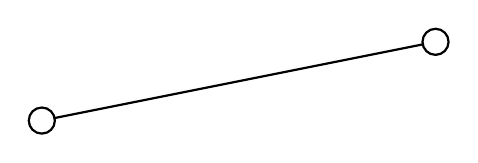
\begin{tikzpicture}
    \draw[thick] 
      (0,0) node[draw=black,fill=white,shape=circle,text=white] {} 
        -- (5,1) node[draw=black,fill=white,shape=circle,text=white] {} 
    ;
  \end{tikzpicture}
  \caption{$K_{2}$ : a fully connected undirected graph with two vertices}
  \label{fig:k2_graph}
\end{figure}

\section{Function to create such a graph}

To create $K_{2}$, the following code can be used:

\lstinputlisting[
  caption = Creating $K_{2}$ as depicted in figure \ref{fig:k2_graph},
  label = lst:create_k2_graph
]{create_k2_graph.impl}

This code is very similar to 
the \verb;add_edge; function (algorithm \ref{lst:add_edge}).
Instead of typing the graph its type, 
we call the \verb;create_empty_undirected_graph; 
function and let auto figure it out.
The vertex descriptors 
(see chapter \ref{subsec:Vertex-descriptors}) 
created by two \verb;boost::add_vertex; \index{boost::add\_vertex}
calls are stored to add an edge to the graph.

From \verb;boost::add_edge; \index{boost::add\_edge}
its return type 
(see chapter \ref{subsec:boost_add_edge_result}), 
it is only checked that insertion has been successful.

Note that the graph lacks all properties: nodes do not have names, nor do
edges.

\section{Creating such a graph}

Listing \ref{lst:create_k2_graph_demo}
demonstrates how to \verb;create_k2_graph; and checks if it has the correct
amount of edges and vertices:

\lstinputlisting[
  caption = Demonstration of create\_k2\_graph
  label = lst:create_k2_graph_demo
]{create_k2_graph_demo.impl}

\section{The .dot file produced}
\label{subsec:create_k2_dot}

Running a bit ahead, this graph can be converted to the .dot file as shown
in algorithm \ref{lst:create_k2_graph.dot}:

\lstinputlisting[
  caption = .dot file created from the create\_k2\_graph function (algorithm \ref{lst:create_k2_graph}) converted from graph to .dot file using algorithm \ref{lst:save_graph_to_dot},
  label = lst:create_k2_graph.dot
]{create_k2_graph.dot}

From the .dot file one can already see that the graph is undirected, because:

\begin{itemize}
  \item The first word, \verb;graph;, denotes an undirected graph 
    (where \verb;digraph; would have indicated a directional graph)
  \item The edge between 0 and 1 is written as \verb;–; 
    (where directed connections would be written as \verb;->;, 
    \verb;<-; or \verb;<>;)
\end{itemize}

\section{The .svg file produced}
\label{subsec:create_k2.svg}

Continuing to running a bit ahead, 
this .dot file can be converted to the .svg 
as shown in figure \ref{fig:create_k2_graph.svg}:

\begin{figure}[!htbp]
  \includegraphics[]{create_k2_graph.png}
  \caption{.svg file created from the create\_k2\_graph' function (algorithm \ref{lst:create_k2_graph}) its .dot file, converted from .dot file to .svg using algorithm \ref{lst:convert_dot_to_svg}}
  \label{fig:create_k2_graph.svg}
\end{figure}

Also this figure shows that the graph in undirected, otherwise the edge
 would have one or two arrow heads.
 The vertices display the node index, which is the default behavior.

%%%%%%%%%%%%%%%%%%%%%%%%%%%%%%%%%%%%%%%%%%%%%%%%%%%%%%%%%%%%%%%%%%%%%%%%%%%%%%%%
\section{$\triangle$ Creating $K_{3}$, a fully connected undirected graph with three vertices}
\label{subsec:create_k3_graph}
\index{Create $K_{3}$}
\index{$K_{3}$, create}
%%%%%%%%%%%%%%%%%%%%%%%%%%%%%%%%%%%%%%%%%%%%%%%%%%%%%%%%%%%%%%%%%%%%%%%%%%%%%%%%

This is an extension of the previous chapter

\section{Graph}

To create a fully connected undirected graph with three vertices 
(also called $K_{4}$), 
one needs three vertices and three (undirected) edge, 
as depicted in figure \ref{fig:create_k3_graph}.

\begin{figure}
  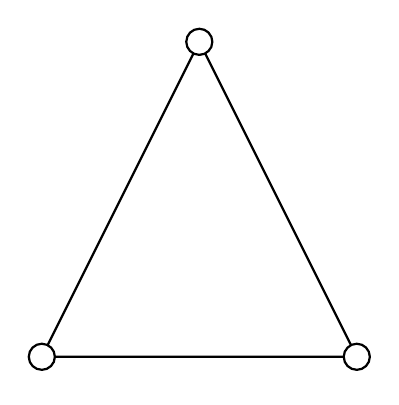
\begin{tikzpicture}
    \draw[thick] 
      (2,4) node[draw=black,fill=white,shape=circle,text=white] {} 
       -- (3,2) node[anchor=west] {} 
       -- (4,0) node[draw=black,fill=white,shape=circle,text=white] {} 
       -- (2,0) node[anchor=north] {} 
       -- (0,0) node[draw=black,fill=white,shape=circle,text=white] {} 
       -- (1,2) node[anchor=east] {} 
       -- (2,4)
    ;
  \end{tikzpicture}
  \caption{$K_{3}$: a fully connected graph with three edges and vertices }
  \label{fig:create_k3_graph}
\end{figure}

\section{Function to create such a graph}

To create $K_{3}$, the following code can be used:

\lstinputlisting[
  caption = Creating $K_{3}$ as depicted in figure \ref{fig:create_k3_graph},
  label = lst:create_k3_graph
]{create_k3_graph.impl}
\index{Create $K_{3}$ graph}

\section{Creating such a graph}

Listing \ref{lst:create_k3_graph_demo} demonstrates 
\verb;create_k3_graph; and checks if it has the correct
amount of edges and vertices:

\lstinputlisting[
  caption = Demonstration of create\_k3\_graph,
  label = lst:create_k3_graph_demo
]{create_k3_graph_demo.impl}

\section{The .dot file produced}
\label{subsec:create_k3_graph.dot}

This graph can be converted to the .dot file as shown in algorithm 
\ref{lst:create_k3_graph.dot}:

\lstinputlisting[
  caption = .dot file created from the create\_k3\_graph function (algorithm \ref{lst:create_k3_graph}) converted from graph to .dot file using algorithm \ref{lst:save_graph_to_dot},
  label = lst:create_k3_graph.dot
]{create_k3_graph.dot}

\section{The .svg file produced}
\label{subsec:create_k3.svg}

Continuing to running a bit ahead, this .dot file can be converted to the
.svg as shown in figure \ref{fig:create_k3_graph.svg}:

\begin{figure}[!htbp]
  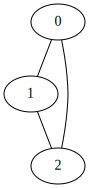
\includegraphics[]{create_k3_graph.png}
  \caption{
    .svg file created from the create\_k3\_graph function 
    (algorithm \ref{lst:create_k3_graph}) its .dot file, 
    converted from .dot file to .svg 
    using algorithm \ref{lst:convert_dot_to_svg}
  }
  \label{fig:create_k3_graph.svg}
\end{figure}

%%%%%%%%%%%%%%%%%%%%%%%%%%%%%%%%%%%%%%%%%%%%%%%%%%%%%%%%%%%%%%%%%%%%%%%%%%%%%%%%
\section{$\triangle$ Creating a path graph}
\label{subsec:create_path_graph}
\index{Create path graph}
\index{Path graph, create}
%%%%%%%%%%%%%%%%%%%%%%%%%%%%%%%%%%%%%%%%%%%%%%%%%%%%%%%%%%%%%%%%%%%%%%%%%%%%%%%%

A path graph is a linear graph without any branches

\section{Graph}

Here I show a path graph with four vertices 
(see figure \ref{fig:create_path_graph}):

\begin{figure}
  \begin{tikzpicture}
    \tikzset{ 
      VertexStyle/.append style = {draw=black,fill=white,shape=circle,text=white}
    }
    \SetGraphUnit{4}
    \Vertex{A}   
    \EA(A){B}   
    \EA(B){C}   
    \EA(C){D}   
    \Edge[](A)(B)   
    \Edge[](B)(C)   
    \Edge[](C)(D)   
  \end{tikzpicture}
  \caption{A path graph with four vertices}
  \label{fig:create_path_graph}
\end{figure}

\section{Function to create such a graph}

To create a path graph, the following code can be used:

\lstinputlisting[
  caption = Creating a path graph as depicted in figure \ref{fig:create_path_graph},
  label = lst:create_path_graph
]{create_path_graph.impl}
\index{Create path graph}

\section{Creating such a graph}

Listing \ref{lst:create_path_graph_demo}
demonstrates \verb;create_path_graph; 
and checks if it has the correct amount of edges and vertices:

\lstinputlisting[
  caption = Demonstration of create\_path\_graph,
  label = lst:create_path_graph_demo
]{create_path_graph_demo.impl}

\section{The .dot file produced}
\label{subsec:create_path_graph.dot}

This graph can be converted to the .dot file 
as shown in algorithm \ref{lst:create_path_graph.dot}:

\lstinputlisting[
  caption = .dot file created from the create\_path\_graph function (algorithm \ref{lst:create_path_graph}) converted from graph to .dot file using algorithm \ref{lst:save_graph_to_dot},
  label = lst:create_path_graph.dot
]{create_path_graph_4.dot}

\section{The .svg file produced}
\label{subsec:create_path_graph.svg}

The .dot file can be converted to the .svg 
as shown in figure \ref{fig:create_path_graph.svg}:

\begin{figure}[!htbp]
  \includegraphics[]{create_path_graph_4.png}
  \caption{
    .svg file created from the create\_path\_graph function 
    (algorithm \ref{lst:create_path_graph}) 
    its .dot file, converted from .dot file to .svg 
    using algorithm \ref{lst:convert_dot_to_svg}
  }
  \label{fig:create_path_graph.svg}
\end{figure}

%%%%%%%%%%%%%%%%%%%%%%%%%%%%%%%%%%%%%%%%%%%%%%%%%%%%%%%%%%%%%%%%%%%%%%%%%%%%%%%%
\section{$\triangle$ Creating a Peterson graph}
\label{subsec:create_petersen_graph}
\index{Create Petersen graph}
\index{Petersen graph, create}
%%%%%%%%%%%%%%%%%%%%%%%%%%%%%%%%%%%%%%%%%%%%%%%%%%%%%%%%%%%%%%%%%%%%%%%%%%%%%%%%

A Petersen graph is the first graph with interesting properties.

\section{Graph}

To create a Petersen graph, one needs five vertices and five undirected
 edges, as depicted in figure 
\ref{fig:create_petersen_graph}.

\begin{figure}[!htbp]
  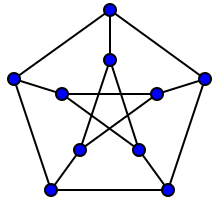
\includegraphics[]{Petersen_graph.png}
  \caption{
    A Petersen graph 
    (from \url{https://en.wikipedia.org/wiki/Petersen_graph}) 
  }
  \label{fig:create_petersen_graph}
\end{figure}

\section{Function to create such a graph}

To create a Petersen graph, the following code can be used:

\lstinputlisting[
  caption = Creating Petersen graph as depicted in figure \ref{fig:create_petersen_graph},
  label = lst:create_petersen_graph
]{create_petersen_graph.impl}
\index{Create Petersen graph}

\section{Creating such a graph}

Listing \ref{lst:create_petersen_graph_demo}
demonstrates how to use \verb;create_petersen_graph' and checks if it has the
correct amount of edges and vertices:

\lstinputlisting[
  caption = Demonstration of create\_k3\_graph,
  label = lst:create_petersen_graph_demo
]{create_petersen_graph_demo.impl}

\section{The .dot file produced}
\label{subsec:create_petersen_graph.dot}

This graph can be converted to the .dot file as shown in algorithm 
\ref{lst:create_petersen_graph.dot}:

\lstinputlisting[
  caption = .dot file created from the create\_petersen\_graph function (algorithm \ref{lst:create_petersen_graph}) converted from graph to .dot file using algorithm \ref{lst:save_graph_to_dot},
  label = lst:create_petersen_graph.dot
]{create_petersen_graph.dot}

\section{The .svg file produced}
\label{subsec:create_petersen.svg}

This .dot file can be converted to the .svg as shown in figure 
\ref{fig:create_petersen_graph.svg}:

\begin{figure}[!htbp]
  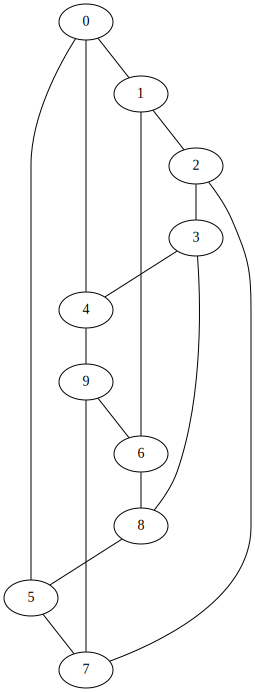
\includegraphics[]{create_petersen_graph.png}
  \caption{
    .svg file created from the create\_petersen\_graph function 
    (algorithm \ref{lst:create_petersen_graph}) its .dot file, 
    converted from .dot file to .svg using algorithm 
    \ref{lst:convert_dot_to_svg}
  }
  \label{fig:create_petersen_graph.svg}
\end{figure}

